\section{Design}
\subsection{Designklassediagram}
\begin{figure}[H]
    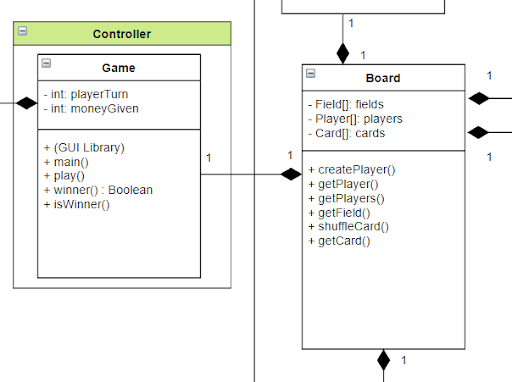
\includegraphics[width=10cm]{figures/Design klasse diagram Game Board}
    \caption{Design klasse diagram udsnit af Game og Board}
\end{figure}
Som der ses på billedet ovenover er vores main metode er i game klassen sammen med reglerne for logik, hvor board er en controller der udfører logik. Man kunne tage main-metoden ud i en separat klasse, men det har vi valgt ikke at gøre, da vi vil have vores main metode i vores game klasse.
Der er valgt at lave nedarvning fra field klassen til Loose Change klassen samt Restroom klassen, da Loose Change klassen og Restroom klassen er deler flere attributter med field klassen dog er de begge lidt forskellige fra field klassen, som ses her:
\begin{figure}[H]
    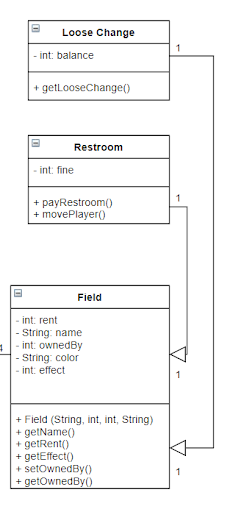
\includegraphics[width=5cm]{figures/Design klasse diagram fields}
    \caption{Design klasse diagram udsnit af Field, Restroom og Loose Change}
\end{figure}
Der er valgt at have en Cup klasse samt en Die klasse hvor Die klassen indeholder en metode der giver et tilfældigt tal mellem 1 og 6 som simulere en rigtig terning. Det er så Cup klassen simulere et raflebæger som slår med terningen ved hjælp af roll metoden hvor der tages to terninger fra Die klassen og skabes 2 værdier. Herefter er der getSum metoden der finder en sum af de to terninger, hvilket er det slag vores spiller har lavet. Dette ses her i design klassediagrammet:
\begin{figure}[H]
    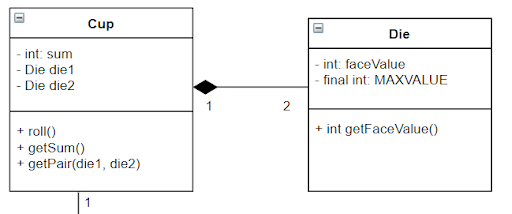
\includegraphics[width=10cm]{figures/Design klasse diagram Cup Die}
    \caption{Design klasse diagram udsnit af Cup og Die}
\end{figure}
Der er valgt at have en player klasse som simulere vores spillere der bliver tildelt navn, farve, placering og ejede grunde med mere. Til player klassen er der koblet en account klasse som styrer spillerens balance, det er også denne attribut der er valgt til i Board klassen at bestemme om en spiller er gået bankerot og derfor har tabt spillet.
\begin{figure}[H]
    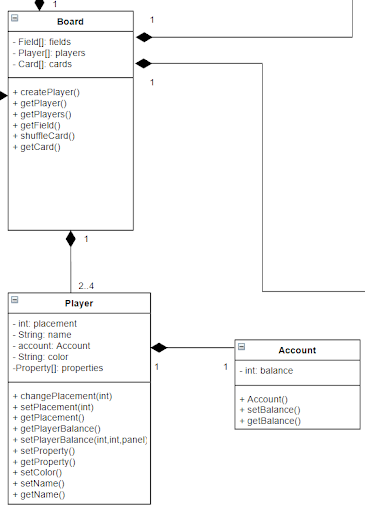
\includegraphics[width=10cm]{figures/Design klasse diagram Board Player Account}
    \caption{Design klasse diagram udsnit af Board, Player og Account}
\end{figure}
\subsection{Sekvensdiagram}
\subsection{GRASP}
\subsubsection{Creator}
\subsubsection{Information Expert}
\subsubsection{Low Coupling High Cohesion}
\subsubsection{Polymorphism}
\subsubsection{Pure Fabrication}
